\documentclass[14pt]{extbook}
\usepackage{multicol, enumerate, enumitem, hyperref, color, soul, setspace, parskip, fancyhdr} %General Packages
\usepackage{amssymb, amsthm, amsmath, latexsym, units, mathtools} %Math Packages
\everymath{\displaystyle} %All math in Display Style
% Packages with additional options
\usepackage[headsep=0.5cm,headheight=12pt, left=1 in,right= 1 in,top= 1 in,bottom= 1 in]{geometry}
\usepackage[usenames,dvipsnames]{xcolor}
\usepackage{dashrule}  % Package to use the command below to create lines between items
\newcommand{\litem}[1]{\item#1\hspace*{-1cm}\rule{\textwidth}{0.4pt}}
\pagestyle{fancy}
\lhead{Progress Quiz 4}
\chead{}
\rhead{Version C}
\lfoot{5346-5907}
\cfoot{}
\rfoot{Summer C 2021}
\begin{document}

\begin{enumerate}
\litem{
Choose the graph of the equation below.\[ f(x) = \frac{1}{x - 1} + 1 \]\begin{enumerate}[label=\Alph*.]
\begin{multicols}{2}\item 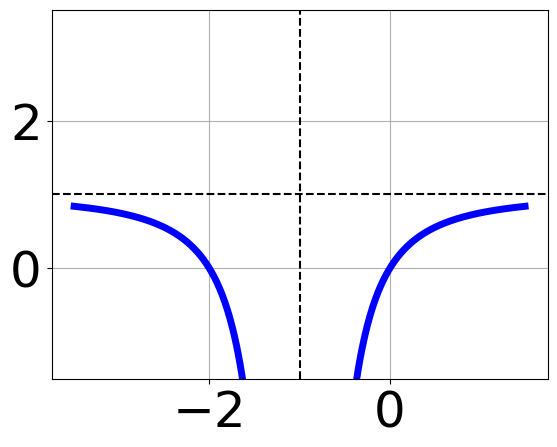
\includegraphics[width = 0.3\textwidth]{../Figures/rationalEquationToGraphAC.png}\item 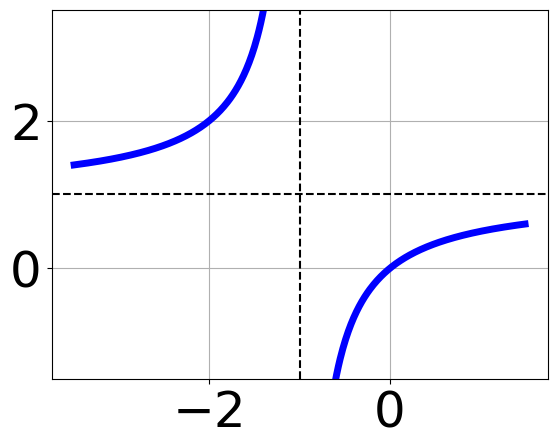
\includegraphics[width = 0.3\textwidth]{../Figures/rationalEquationToGraphBC.png}\item 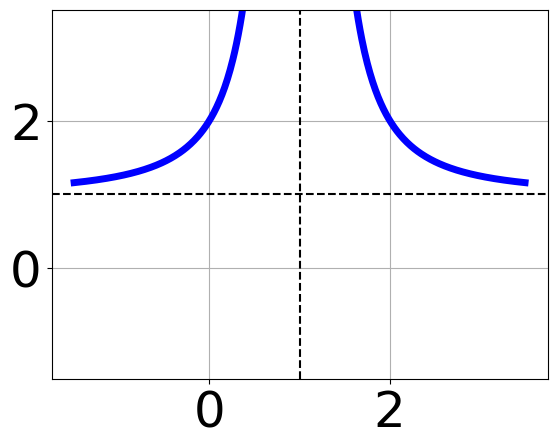
\includegraphics[width = 0.3\textwidth]{../Figures/rationalEquationToGraphCC.png}\item 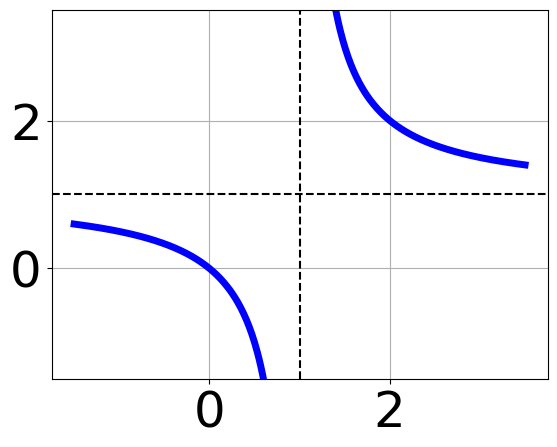
\includegraphics[width = 0.3\textwidth]{../Figures/rationalEquationToGraphDC.png}\end{multicols}\item None of the above.
\end{enumerate} }
\litem{
Choose the equation of the function graphed below.
\begin{center}
    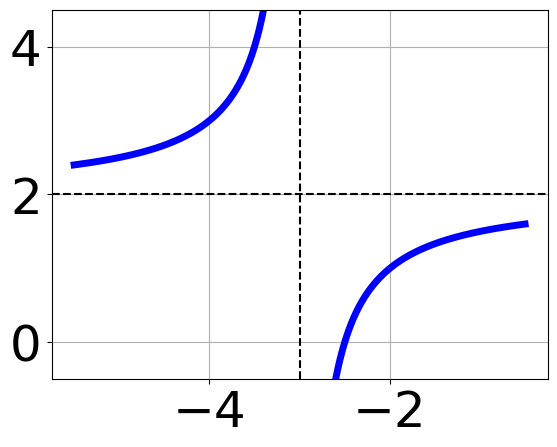
\includegraphics[width=0.5\textwidth]{../Figures/rationalGraphToEquationCopyC.png}
\end{center}
\begin{enumerate}[label=\Alph*.]
\item \( f(x) = \frac{1}{x - 3} + 2 \)
\item \( f(x) = \frac{-1}{x + 3} + 2 \)
\item \( f(x) = \frac{-1}{(x + 3)^2} + 2 \)
\item \( f(x) = \frac{1}{(x - 3)^2} + 2 \)
\item \( \text{None of the above} \)

\end{enumerate} }
\litem{
Choose the equation of the function graphed below.
\begin{center}
    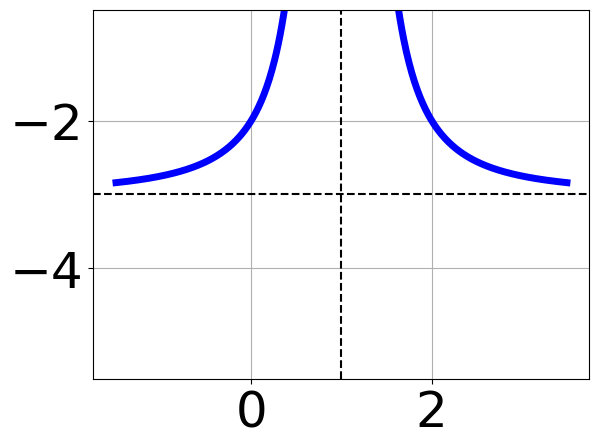
\includegraphics[width=0.5\textwidth]{../Figures/rationalGraphToEquationC.png}
\end{center}
\begin{enumerate}[label=\Alph*.]
\item \( f(x) = \frac{-1}{x - 1} + 4 \)
\item \( f(x) = \frac{-1}{(x - 1)^2} + 4 \)
\item \( f(x) = \frac{1}{(x + 1)^2} + 4 \)
\item \( f(x) = \frac{1}{x + 1} + 4 \)
\item \( \text{None of the above} \)

\end{enumerate} }
\litem{
Solve the rational equation below. Then, choose the interval(s) that the solution(s) belongs to.\[ \frac{-39}{-78x -39} + 1 = \frac{-39}{-78x -39} \]\begin{enumerate}[label=\Alph*.]
\item \( x_1 \in [-0.6, 0.2] \text{ and } x_2 \in [-0.3,2.1] \)
\item \( x \in [-0.5,0.5] \)
\item \( \text{All solutions lead to invalid or complex values in the equation.} \)
\item \( x \in [0.3,1.4] \)
\item \( x_1 \in [-0.6, 0.2] \text{ and } x_2 \in [-0.6,-0.2] \)

\end{enumerate} }
\litem{
Solve the rational equation below. Then, choose the interval(s) that the solution(s) belongs to.\[ \frac{6x}{6x + 6} + \frac{-4x^{2}}{-12x^{2} -36 x -24} = \frac{5}{-2x -4} \]\begin{enumerate}[label=\Alph*.]
\item \( x_1 \in [-3.46, -2.65] \text{ and } x_2 \in [-1.06,-0.71] \)
\item \( x_1 \in [-3.46, -2.65] \text{ and } x_2 \in [-0.77,-0.49] \)
\item \( x \in [-2.32,-0.88] \)
\item \( \text{All solutions lead to invalid or complex values in the equation.} \)
\item \( x \in [-1.35,0.49] \)

\end{enumerate} }
\litem{
Determine the domain of the function below.\[ f(x) = \frac{3}{12x^{2} +29 x + 15} \]\begin{enumerate}[label=\Alph*.]
\item \( \text{All Real numbers except } x = a \text{ and } x = b, \text{ where } a \in [-15.6, -13.6] \text{ and } b \in [-13.9, -11.7] \)
\item \( \text{All Real numbers except } x = a, \text{ where } a \in [-1.7, -1.5] \)
\item \( \text{All Real numbers except } x = a \text{ and } x = b, \text{ where } a \in [-1.7, -1.5] \text{ and } b \in [-0.8, -0.2] \)
\item \( \text{All Real numbers.} \)
\item \( \text{All Real numbers except } x = a, \text{ where } a \in [-15.6, -13.6] \)

\end{enumerate} }
\litem{
Solve the rational equation below. Then, choose the interval(s) that the solution(s) belongs to.\[ \frac{84}{98x -98} + 1 = \frac{84}{98x -98} \]\begin{enumerate}[label=\Alph*.]
\item \( x_1 \in [-1.3, 0.3] \text{ and } x_2 \in [0,3] \)
\item \( \text{All solutions lead to invalid or complex values in the equation.} \)
\item \( x_1 \in [0.4, 1.8] \text{ and } x_2 \in [0,3] \)
\item \( x \in [1.0,2.0] \)
\item \( x \in [-1.3,0.3] \)

\end{enumerate} }
\litem{
Solve the rational equation below. Then, choose the interval(s) that the solution(s) belongs to.\[ \frac{4x}{-5x + 6} + \frac{-4x^{2}}{-15x^{2} +28 x -12} = \frac{3}{3x -2} \]\begin{enumerate}[label=\Alph*.]
\item \( x \in [0.97,1.79] \)
\item \( x_1 \in [-2.15, -1.77] \text{ and } x_2 \in [1.17,1.24] \)
\item \( x_1 \in [-2.15, -1.77] \text{ and } x_2 \in [1.04,1.13] \)
\item \( \text{All solutions lead to invalid or complex values in the equation.} \)
\item \( x \in [0.33,0.72] \)

\end{enumerate} }
\litem{
Choose the graph of the equation below.\[ f(x) = \frac{1}{x + 2} - 3 \]\begin{enumerate}[label=\Alph*.]
\begin{multicols}{2}\item 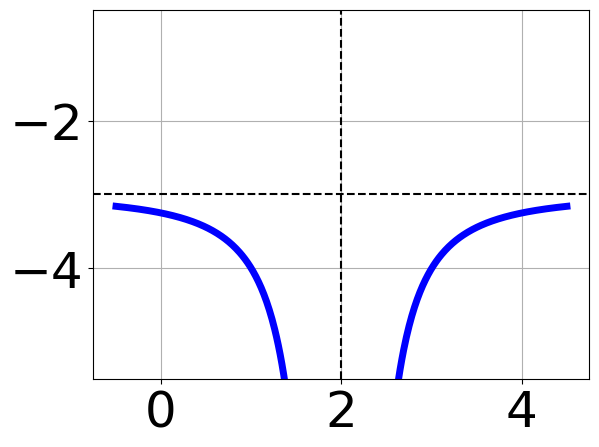
\includegraphics[width = 0.3\textwidth]{../Figures/rationalEquationToGraphCopyAC.png}\item 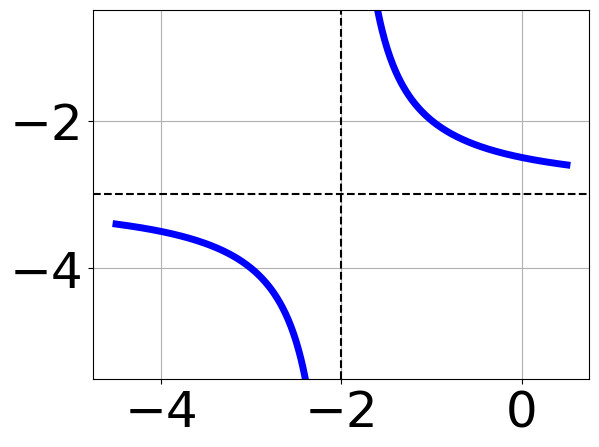
\includegraphics[width = 0.3\textwidth]{../Figures/rationalEquationToGraphCopyBC.png}\item 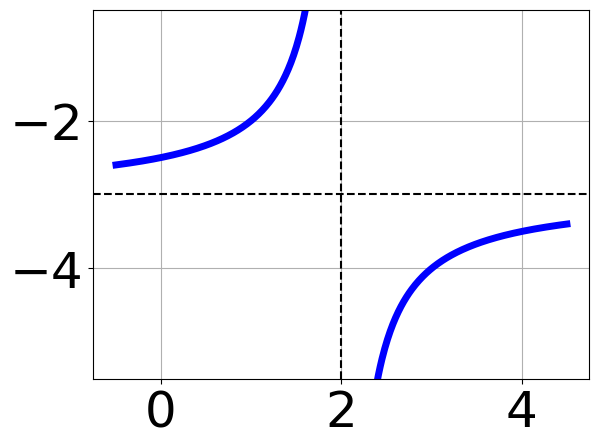
\includegraphics[width = 0.3\textwidth]{../Figures/rationalEquationToGraphCopyCC.png}\item 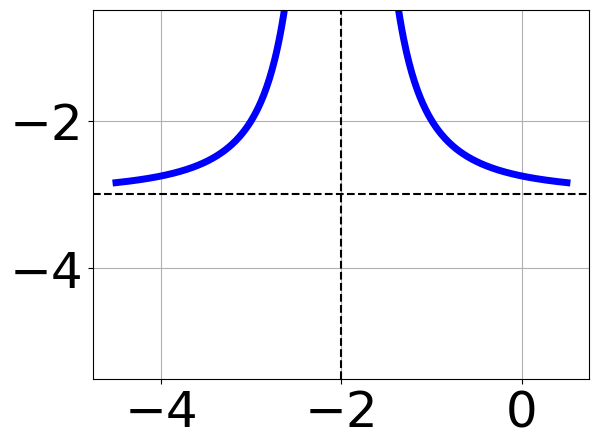
\includegraphics[width = 0.3\textwidth]{../Figures/rationalEquationToGraphCopyDC.png}\end{multicols}\item None of the above.
\end{enumerate} }
\litem{
Determine the domain of the function below.\[ f(x) = \frac{4}{30x^{2} -49 x + 20} \]\begin{enumerate}[label=\Alph*.]
\item \( \text{All Real numbers except } x = a, \text{ where } a \in [19.95, 20] \)
\item \( \text{All Real numbers except } x = a \text{ and } x = b, \text{ where } a \in [0.78, 0.83] \text{ and } b \in [0.82, 0.84] \)
\item \( \text{All Real numbers.} \)
\item \( \text{All Real numbers except } x = a \text{ and } x = b, \text{ where } a \in [19.95, 20] \text{ and } b \in [29.98, 30.02] \)
\item \( \text{All Real numbers except } x = a, \text{ where } a \in [0.78, 0.83] \)

\end{enumerate} }
\end{enumerate}

\end{document}